\documentclass[10pt, mathserif]{beamer}

\usepackage[utf8]{inputenc}
\usepackage[russian]{babel}

\usepackage{listings}
\usepackage{color}
\usepackage{amssymb, amsmath}
\usepackage[all]{xy}
\usepackage{alltt}
\usepackage{pslatex}
\usepackage{epigraph}
\usepackage{verbatim}
\usepackage{graphicx}
\usepackage{latexsym}
\usepackage{array}
\usepackage{changepage} % for adjustwidth
\usepackage{pstricks}
\usepackage{tikz}
\usepackage{pdfpages}
\usepackage{fontawesome}
\usepackage[scaled]{DejaVuSansMono}
\usepackage[T1]{fontenc}


\makeatletter
\newcolumntype{e}[1]{%--- Enumerated cells ---
   >{\minipage[t]{\linewidth}%
     \NoHyper%                Hyperref adds a vertical space
     \let\\\tabularnewline
     \enumerate
        \addtolength{\rightskip}{0pt plus 50pt}% for raggedright
        \setlength{\itemsep}{-\parsep}}%
   p{#1}%
   <{\@finalstrut\@arstrutbox\endenumerate
     \endNoHyper
     \endminipage}}

\newcolumntype{i}[1]{%--- Itemized cells ---
   >{\minipage[t]{\linewidth}%
        \let\\\tabularnewline
        \itemize
           \addtolength{\rightskip}{0pt plus 50pt}%
           \setlength{\itemsep}{-\parsep}}%
   p{#1}%
   <{\@finalstrut\@arstrutbox\enditemize\endminipage}}

\AtBeginDocument{%
    \@ifpackageloaded{hyperref}{}%
        {\let\NoHyper\relax\let\endNoHyper\relax}}
\makeatother

\definecolor{shadecolor}{gray}{1.00}
\definecolor{darkgray}{gray}{0.30}

\newcommand{\set}[1]{\{#1\}}
\newcommand{\angled}[1]{\langle {#1} \rangle}
\newcommand{\fib}{\rightarrow_{\mathit{fib}}}
\newcommand{\fibm}{\Rightarrow_{\mathit{fib}}}
\newcommand{\oo}[1]{{#1}^o}
\newcommand{\inml}[1]{\mbox{\lstinline{#1}}}

\setlength{\epigraphwidth}{.55\textwidth}

\definecolor{light-gray}{gray}{0.90}
\newcommand{\graybox}[1]{\colorbox{light-gray}{#1}}

\newcommand{\nredrule}[3]{
  \begin{array}{cl}
    \textsf{[{#1}]}&
    \begin{array}{c}
      #2 \\
      \hline
      \raisebox{-1pt}{\ensuremath{#3}}
    \end{array}
  \end{array}}

\newcommand{\naxiom}[2]{
  \begin{array}{cl}
    \textsf{[{#1}]} & \raisebox{-1pt}{\ensuremath{#2}}
  \end{array}}


\newcommand\Wider[2][3em]{%
\makebox[\linewidth][c]{%
  \begin{minipage}{\dimexpr\textwidth+#1\relax}
  \raggedright#2
  \end{minipage}
  }%
}

\lstdefinelanguage{ocaml}{
keywords={let, begin, end, in, match, type, and, fun, module,
function, try, with, class, object, method, of, rec, repeat, until,
while, not, do, done, as, val, inherit, module, sig, @ type, struct,
if, then, else, open, virtual, new, fresh},
sensitive=true,
basicstyle=\small\ttfamily,
commentstyle=\scriptsize\rmfamily,
keywordstyle=\ttfamily\bfseries,
identifierstyle=\ttfamily,
basewidth={0.5em,0.5em},
columns=fixed,
fontadjust=true,
literate={->}{{$\to$}}1
         {===}{{$\equiv$}}1
         {=/=}{{$\not\equiv$}}1
}

\lstdefinelanguage{scheme}{
keywords={define, conde, fresh},
sensitive=true,
basicstyle=\small,
commentstyle=\scriptsize\rmfamily,
keywordstyle=\ttfamily\bfseries,
identifierstyle=\ttfamily,
basewidth={0.5em,0.5em},
columns=fixed,
fontadjust=true,
literate={==}{{$\equiv$}}1
}

\lstset{
basicstyle=\small,
identifierstyle=\ttfamily,
keywordstyle=\bfseries,
commentstyle=\scriptsize\rmfamily,
basewidth={0.5em,0.5em},
% fontadjust=true,
escapechar=!,
language=ocaml
}

\setbeamertemplate{footline}[frame number]
\setbeamertemplate{navigation symbols}{}
\setbeamertemplate{blocks}[rounded][shadow=true]
\beamertemplateballitem

\mode<presentation>{
  \usetheme{default}
}

\AtBeginSection[]
{
\begin{frame}{Table of Contents}
\tableofcontents[currentsection]
\end{frame}
}
\theoremstyle{definition}

\title{Copattern matching and first-class observations in OCaml, with a macro}
\author{Дмитрий Косарев}

\date{
  \vskip 2cm
  \small{
    \textbf{19 февраля, 2018}
  }
}


% some slides https://www.cl.cam.ac.uk/events/metaprog2016/codata-types-and-copattern-matching.pdf
% original paper https://hal.inria.fr/hal-01653261/document
\begin{document}
\begin{frame}
  \titlepage
\end{frame}


\section{Мотивация}

\begin{frame}{Спойлер?}
\begin{itemize}
 \item Расширим OCaml копаттернами, кофункциями и т.д.
\end{itemize}

\end{frame}

\begin{frame}{Мотивация}
 
\begin{itemize}
  \item Конечные
  \begin{itemize}
    \item Например: список, дерево, ...
    \item Индуктивные типы и pattern matching
  \end{itemize}
  \item Бесконечные
  \begin{itemize}
    \item Например: stream, бесконечное дерево, ...
    \item Коиндуктивные типы и copattern matching
  \end{itemize}
  \vspace{1in}
  \pause
  Copatterns: Programming Infinite Structures by Observations
  Abel, Pientka, Thibodeau and Setzer (POPL – 2013)
\end{itemize}

\end{frame}

\begin{frame}[fragile]{Data types and Pattern matching}
A data type is defined by its Constructors :

\begin{lstlisting}[language=ocaml,mathescape=true]
type 'a list = Nil | Cons of 'a * 'a list

let ns: int list = Cons(1, Cons(2,Nil))
\end{lstlisting}
Deconstruct with pattern matching:
\begin{lstlisting}[language=ocaml,mathescape=true]
let rec map f xs =
  match xs with
  | Nil -> Nil
  | Cons (x,xs) -> Cons(f x, map f xs)

map succ ns;;

$-$ : int list = Cons(2, Cons(3, Nil))
\end{lstlisting}
\end{frame}

\begin{frame}[fragile]{Мотивация}
\begin{itemize}
 \item Call-by-value is an evaluation strategy in which the arguments are evaluated before being passed to the functions.
\begin{lstlisting}
let rec zeros = Cons (0, zeros )
\end{lstlisting}
Вычисление расходится
\item Решение - ?
\end{itemize}
\end{frame}

\begin{frame}[fragile]{Мотивация}
Call-by-value $\Rightarrow$ раходимость.

Решение : сэмулировать call-by-name (à la Haskell). 


\begin{lstlisting}[language=ocaml,mathescape=true]
type 'a list = Nil | Cons of 'a * (unit -> 'a list)

let rec zeros = Cons (0, fun () -> zeros)
\end{lstlisting}

\begin{lstlisting}[language=ocaml,mathescape=true]
let rec map f xs =
  match xs with
  | Nil -> Nil
  | Cons (x,th) -> Cons(f x, map f (th ()))

map ((+)1) zeros;;

$-$ : int list = Cons(1, <fun>)
\end{lstlisting}
\end{frame}


\section{GADT}


\begin{frame}{Реляционное программирование на miniKanren}
 % \vskip1cm
 \begin{center}
 От программ-\emph{функций} к программам-\emph{отношениям}:
 \end{center}

 $$
 f \colon X \to Y\;\leadsto\;\oo{f} \subseteq X\times Y
 $$
 \vskip5mm
 \begin{tabular}{m{4cm}m{6cm}}
    %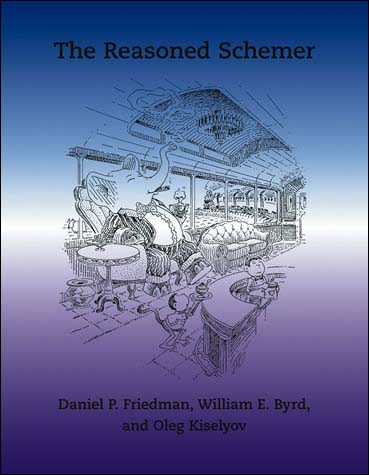
\includegraphics[scale=0.3]{trs.jpg} &
    \begin{itemize}
       \item Изначально DSL для Scheme/Racket с довольно минималистичной реализацией
       \item Семейство языков ($\mu$Kanren, $\alpha$  Kanren, cKanren, и т.д.)
       \item Встраивается как DSL в широкий набор языков (включая OCaml, Haskell, Scala, и т.д.)
       \item Daniel P. Friedman, William Byrd and   Oleg Kiselyov. \emph{The Reasoned Schemer},
       The MIT Press, Cambridge, MA, 2005
    \end{itemize}
 \end{tabular}
 \vskip 3cm
\end{frame}

\begin{frame}[fragile]{Пример: реляционное слияние списков (OCaml/OCanren/miniKanren)}
%\vskip5mm
\begin{adjustwidth}{-1.5em}{-1.5em}
\begin{tabular}{m{6cm}m{6cm}}
 \graybox{$\inml{append} \colon \alpha\:\inml{list} \to \alpha\:\inml{list} \to \alpha\:\inml{list}$} &
 \graybox{$\oo{\inml{append}}\subseteq\alpha\:\inml{list}\times\alpha\:\inml{list}\times\alpha\:\inml{list}$}\\
 \begin{lstlisting}[language=ocaml,keywordstyle=\bfseries]
let rec append xs ys =
  match xs with
  | []      -> ys
  | h :: tl ->
      h :: (append tl ys)!\pause!
 \end{lstlisting} &
 \begin{lstlisting}[mathescape=true,language=ocaml]
let rec append$^o$ xs ys xys =!\pause!
  ((xs === nil) &&& (xys === ys))!\pause!
  |||
  (fresh (h t tys)!\pause!
     (xs  === h % t)!\pause!
     (xys === h % tys)!\pause!
     (append$^o$ t ys tys) )
 \end{lstlisting}
\end{tabular}\pause
\begin{center}
\begin{minipage}{6cm}
\centering{\small\bf В оригинальной реализации:}
\begin{lstlisting}[mathescape=true,language=scheme]
(define (append$^o$ xs ys xys)
   (conde
      [(== '() xs) (== ys xys)]
      [(fresh (h t tys)
         (== `(,h . ,t) xs)
         (== `(,h . ,tys) xys)
         (append$^o$ t ys tys))]))
\end{lstlisting}
\end{minipage}
\end{center}

\end{adjustwidth}
\vskip5mm
\end{frame}

% \begin{frame}[fragile]{Набросок минимальной реализации}
% Jason Hemann, Daniel P. Friedman. \emph{$\mu$Kanren: A Minimal Functional
% Core for Relational Programming} // Scheme'13:
% \vskip5mm
% \small
% \pause
% \begin{tabular}{p{5cm}c}
% Логические переменные  & $X=\{x_1,x_2,\dots\}$ \vspace*{-\baselineskip} \\
% Символы (конструкторы) & $S=\{s_1,s_2,\dots\}$ \vspace*{-\baselineskip} \\
% Термы                  & $T=X\cup\{s\;(t_1,\dots,t_k)\mid s\in S,\; t_i \in T\}$ \vspace*{-\baselineskip} \\
% Подстановки            & $\Sigma=T^X$ \vspace*{-\baselineskip} \\
% \\\pause
% Унификация & $(\equiv)\colon\Sigma\to T\to T\to\Sigma_\perp$ \vspace*{-\baselineskip}\\
% \\\pause
% State (подстановка + как создавать новые логические переменные) & $\sigma$ \vspace*{-\baselineskip}\\
% Goal (функция из состояния в ленивый список состояний) & $g : \sigma\to\sigma\;\inml{stream}$ \vspace*{-\baselineskip} \\
% Конъюнкция $g \wedge g$ & ``bind''  \vspace*{-\baselineskip} \\
% Дизъюнкция $g \vee   g$ & ``mplus'' \vspace*{-\baselineskip} \\
% 
% Refinement: извлечение посчитанных ответов & $\inml{refine} \colon \sigma\to X\to T$ \vspace*{-\baselineskip}
% \end{tabular}
% 
% \end{frame}

\begin{frame}[fragile]{miniKanren vs. Prologs (1)}
\begin{itemize}
  \item Стратегия поиска: interleaving.
%       \begin{itemize}
% 	\item Поиск в глубину (DFS) быстрее при конечном переборе.
% 	\item Чтобы DFS завершался в Prolog введены дополнительные синтаксические конструкции (cuts).
%       \end{itemize}
%   \item miniKanren реализован как DSL -- встраивается в другие языки.
\end{itemize}
\end{frame}

\begin{frame}[fragile]{Поиск в глубину (dfs)}
\begin{figure}
\centering
%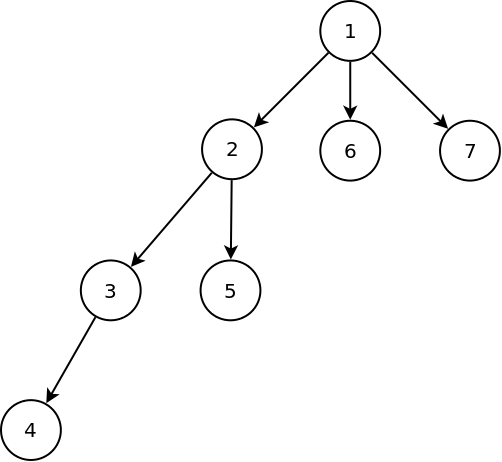
\includegraphics[width=0.7\textwidth]{dfs.png}
\end{figure}
\end{frame}

\begin{frame}[fragile]{Поиск в ширину (bfs)}
\begin{figure}
\centering
%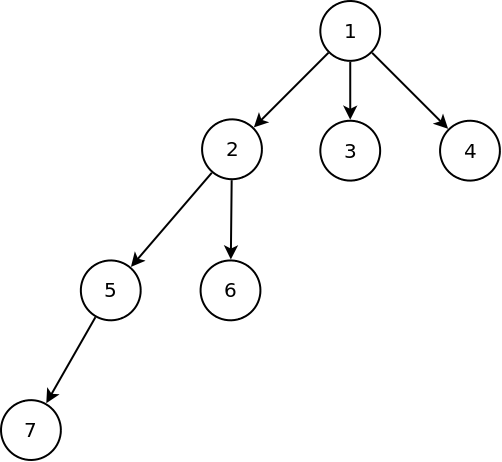
\includegraphics[width=0.7\textwidth]{bfs.png}
\end{figure}
\end{frame}

\begin{frame}[fragile]{Interleaving поиск}
\begin{figure}
\centering
%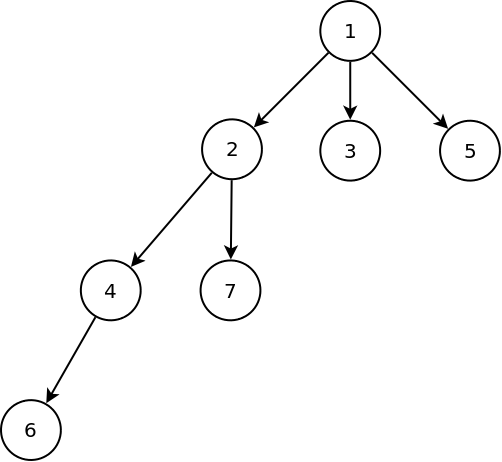
\includegraphics[width=0.7\textwidth]{interleave.png}
\end{figure}
\end{frame}

\begin{frame}[fragile]{miniKanren vs. Prologs (2)}
\begin{itemize}
  \item Стратегия поиска: interleaving search.
      \begin{itemize}
	\item Поиск в глубину (DFS) быстрее при конечном переборе.
	\item Чтобы DFS завершался в Prolog введены дополнительные синтаксические конструкции (cuts).
      \end{itemize}
  \item miniKanren реализован как DSL -- встраивается в другие языки.
\end{itemize}
\end{frame}

\begin{frame}[fragile]{Цель работы}
OCanren -- DSL для типобезопасного встраивания miniKanren в OCaml.
\end{frame}

\begin{frame}[fragile]{Изначальные ожидания}
\begin{itemize}
 \item Меньше ошибок при разработке.
 \item Сходная производительность, или даже лучше.
\end{itemize}

\end{frame}

\begin{frame}[fragile]{Предыдущие типобезопасные встраивания}
\begin{itemize}
 \item HaskellKanren    \href{https://github.com/JaimieMurdock/HK}{\faGithub}
 \item ukanren          \href{https://github.com/rntz/ukanren}{\faGithub}
 \item miniKanren-ocaml \href{https://github.com/lightyang/minikanren-ocaml}{\faGithub}
 \item Molog            \href{https://github.com/acfoltzer/Molog}{\faGithub}
 \item MiniKanrenT      \href{https://github.com/jvranish/MiniKanrenT}{\faGithub}
\end{itemize}
\pause
\vspace{1in}
Различия могу быть в следущем:
\begin{itemize}
 \item Как именно используются типы?
 \item Как производится унификация?
\end{itemize}

\end{frame}



\begin{frame}[fragile]{Как используются типы?}
\begin{itemize}
\item Один заранее созданный тип, на котором унификация разрешена.
  \begin{itemize}
    \item[\faTimes] Нет поддержки пользовательских типов.

    \item[\faCheck] ``Универсальная'' функция унификации.
  \end{itemize}
    \vspace{1em}
    ukanren, miniKanren-ocaml, HaskellKanren
    \vspace{1em}
\pause
\item О размещении логических переменных беспокоится пользователь.
  \begin{itemize}
    \item[\faTimes] Неудобно.
    \item[\faTimes] Функция унификации для каждого типа своя.
    \item[\faCheck] Поддержка произвольных типов данных.
  \end{itemize}
  \vspace{1em}
  miniKanrenT, Molog
\end{itemize}
\end{frame}

\begin{frame}[fragile]{Как сделано в OCanren?}

\begin{itemize}
 \item Один тип для разделения логических переменных от конкретных термов
    \begin{lstlisting}[mathescape=true]
      type $\alpha$ logic = Var of int | Value of $\alpha$
    \end{lstlisting}
 \item который используется в пользовательских типах.

 \pause
 \item Полиморфная унификация -- \emph{одна} для всех типов.
 % Почему-то курсив не работает
    \vspace{1em}
    \begin{itemize}
    \item[\faTimes] Подход специфичен для OCaml.
    \item[\faTimes] Написано в типонебезопасном стиле...
    \item[\faCheck] ... но это скрыто от пользователя.
    \item[\faCheck] Идеалогически как в первоисточнике.
    \end{itemize}
  \pause
  \item Пользователь должен следовать рекомендациям по описанию типов.
\end{itemize}
\end{frame}

\begin{frame}[fragile]{Систематическое конструирование логических типов (на примере списка)}
  % mathescape=true,
  \begin{lstlisting}[mathescape=true]
  type $\alpha$ logic = Var of int | Value of $\alpha$
  ...!\pause!
  type ($\alpha$, $\beta$) glist = Nil | Cons of $\alpha$ * $\beta$ !\pause!

  type $\alpha$  list = ($\alpha$, $\alpha$ list) glist !\pause!

  type $\alpha$ llist = ($\alpha$, $\alpha$ llist) glist logic !\pause!

  ...
  # Value Nil
  -: $\alpha$ llist
  # Value (Cons (Value 1), Value Nil)
  -: int logic llist
  # Value (Cons (Var 101), Value Nil)
  -: int logic llist
  \end{lstlisting}
\end{frame}


\begin{frame}[fragile]{Типобезопасность (пример)}
\begin{lstlisting}[mathescape=true]
type $\alpha$ logic = Var of int | Value of $\alpha$
...
val x : $\alpha$ logic
val s : string logic
...
(x === s)
...
!\pause!
val n : int logic
... (x === n) ...
\end{lstlisting}
\begin{verbatim}
Error: 
  This expression has type int logic
  but an expression was expected of type string logic
  Type int is not compatible with type string
\end{verbatim}

\end{frame}

\begin{frame}[fragile]{Промежуточные результаты}
Были представлены на ML Workshop 2016 (совмещённым с ICFP 2016)
\begin{itemize}
\item Типобезопасное встраивание miniKanren в OCaml.
\item Полиморфная унификация.
\item Подход для описания типов.
\end{itemize}

\vspace{2em}
\pause
\begin{enumerate}
 \item[\faCheck] Типы помогают выявить некоторые ошибки.
 \pause
 \item[\faTimes] Выигрыша в скорости нет.
 \item[\faTimes] Даже наоборот.
\end{enumerate}

\end{frame}

\begin{frame}[fragile]{Дальнейшие задачи}
  \begin{itemize}
  \item Найти причину замедления.
  \item Ускорить.
  \item Подход должен остаться типобезопасным.
  \end{itemize}

\end{frame}

\begin{frame}[fragile]{Полиморфная унификация в OCanren}

Работает для всех логических типов  $\oo{\alpha}$:

$$
(\equiv)\;\colon \Sigma\to\oo{\alpha}\to\oo{\alpha}\to\Sigma_{\perp}
$$
\pause

Стандартный алгоритм с треугольной подстановкой и \textit{occurs check}, использующий типонебезопасный интерфейс  \lstinline{Obj}.
\pause

\vspace{3em}
Тонкости:
\begin{itemize}
\item Типонебезопасный стиль -- компилятор теряет информацию о типах.
\item Дополнительная стадия восстановления типов (refinement).
\end{itemize}
\end{frame}

% \begin{frame}[fragile]{Полиморфная унификация 2 из 7}
%   %\begin{figure}
%   \centering
%   %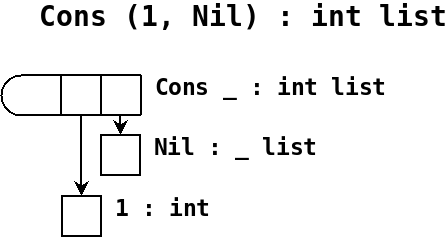
\includegraphics[width=0.6\textwidth]{img0.pdf}
%   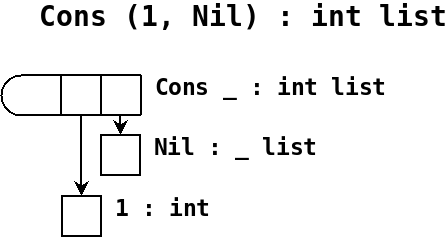
\includegraphics[scale=0.5]{img0.png}
%   %\end{figure}
% \end{frame}

\begin{frame}[fragile]{Алгебраические типы данных в памяти}
  \centering
  \begin{lstlisting}[mathescape=true]
    type ($\alpha, \beta, ...$) typ =   
    | $C_1$ of $t_{11}$ * ... * $t_{1m}$  
    | ...
    | $C_n$ of $t_{n1}$ * ... * $t_{nm}$  
  \end{lstlisting}
  \pause
  \vspace{3em}
  

\end{frame}



\begin{frame}[fragile]{План улучшения реализации}
  \begin{itemize}
  \item Новое представление деревьев
    \begin{itemize}
      \item Значению нельзя присвоить конкретный тип.
      \item Нужен абстрактный тип значений.
      \item Предоставить интерфейс для конструирования логических значений.
      \item Преобразование абстрактного логического значения в типизируемое (во время refinement).
    \end{itemize}
  \item Модернизировать подход по описанию типов логических значений.
  \item Не потерять типовую безопасность.
  \end{itemize}
\end{frame}

\begin{frame}[fragile]{Тип injected}
  \begin{lstlisting}[mathescape=true]
  type ($\alpha$, $\beta$) injected!
  \end{lstlisting}

\vskip 1cm
  Тип $\alpha$ -- это исходный тип, а тип $\beta$ -- его логическое представление
% \vskip 1cm
%   Представление ground-типов совпадает с представлением $\alpha$.
\end{frame}

\begin{frame}[fragile]{Конструирование логических значений для простых типов}
  \begin{lstlisting}[mathescape=true]
  type ($\alpha$, $\beta$) injected

  val lift: $\alpha$ ->   ($\alpha$,$\alpha$) injected
  val inj : ($\alpha$, $\beta$) injected -> $\thinspace$  ($\alpha$, $\beta$ logic) injected
  \end{lstlisting}
  \pause\vskip 1cm
  Например, для чисел:
  \begin{lstlisting}[mathescape=true]
  # inj (lift 5)
  -: (int, int logic) injected
  \end{lstlisting}
  \pause
  Оба введенных примитива оставляют переданное значение как есть (identity)
\end{frame}

\begin{frame}[fragile]{Конструирование логических значений для сложных типов}
  \begin{lstlisting}[mathescape=true]
  module Option = struct
    type $\alpha$ option = None | Some of $\alpha$
    let fmap = ...
  end!\pause!

  # Make1(Option).distrib
  ...!\pause!
  # let some x  = inj (distrib (Some x))
  -: ($\alpha$, $\beta$) injected -> $\thinspace$ ($\alpha$ option, $\beta$ option logic) injected
  \end{lstlisting}
  \pause

  Примитив \lstinline{distrib}, который позволяет конструировать из значений типа \lstinline{(_, _) injected} 
  другие значения типа \lstinline{(_, _) injected}.
  \vskip 1cm
  Он ничего не делает со значением (identity).
  
%   Здесь \emph{fmap} нужен для доказательства того, что тип является функтором, т.е.
%   что \emph{distrib} можно приминить.

\end{frame}

\begin{frame}[fragile]{Восстановление посчитанных значений (refinement)}
  Необходимо, так как значения в типе \lstinline[mathescape=true]{($\alpha$, $\beta$) injected} хранятся в
  нетипизированном виде.

  \begin{lstlisting}[mathescape=true]
  module Option = struct
    type $\alpha$ option = None | Some of $\alpha$
    let fmap = ...
  end!

  \pause!

  # Make1(Option).reify
    : (($\alpha$, $\beta$) injected -> $\enspace \beta$) -> !\pause!
      ($\alpha$ option, $\beta$ option logic) injected -> 
      $\beta$ option logic

  \end{lstlisting}

  При построении \emph{reify} функция \emph{fmap} используется по существу.
\end{frame}

\begin{frame}[fragile]{Итоговые результаты}

\begin{itemize}
 \item Типобезопасная реализация.
 \item C поддержкой неравенств термов (disequality constraints) и occurs check.
 \item Сравнима по скорости с \href{https://github.com/michaelballantyne/faster-miniKanren/}{faster-miniKanren \faGithub}.
 \item Типы выявляют простые ошибки.
 \item Типобезопасность могут заменить некоторые проверки во время выполнения (abstento, numero, symbolo)...
 \item ... сокращая количество примитивов с 8 до 5 
 (\lstinline{===}, \lstinline{=/=}, конъюнкция, дизъюнкция, fresh).
\end{itemize}

\vskip 2cm
Репозиторий \href{https://github.com/dboulytchev/OCanren}{\faGithub}
\end{frame}

\end{document}
